\documentclass{article}
\usepackage{tikz}
\usetikzlibrary{arrows.meta}

\begin{document}

\begin{figure}[h]
    \centering
    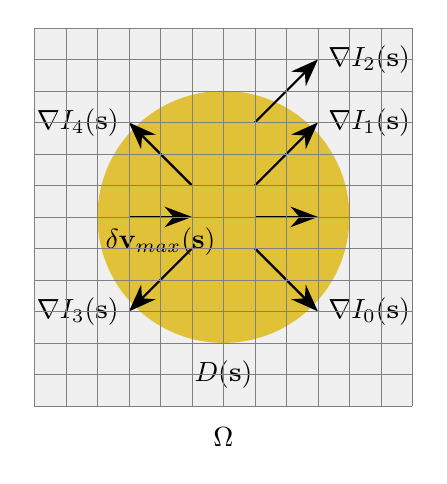
\begin{tikzpicture}[scale=0.8]
        % Define colors
        \definecolor{lightgray}{RGB}{240,240,240}
        \definecolor{darkgray}{RGB}{169,169,169}
        
        % Draw the background rectangle
        \fill[lightgray] (-3,-3) rectangle (3,3);
        
        % Draw the circle
        \fill[yellow!50!brown] (0,0) circle (2cm);
        
        % Draw the vector arrows
        \draw[-{Stealth[scale=1.5]}, thick] (-1.5,0) -- (-0.5,0) node[midway, below] {$\delta \mathbf{v}_{\text{max}}(\mathbf{s})$};
        \draw[-{Stealth[scale=1.5]}, thick] (0.5,0) -- (1.5,0);
        \draw[-{Stealth[scale=1.5]}, thick] (0.5,1.5) -- (1.5,2.5) node[right] {$\nabla I_{2}(\mathbf{s})$};
        \draw[-{Stealth[scale=1.5]}, thick] (0.5,0.5) -- (1.5,1.5) node[right] {$\nabla I_{1}(\mathbf{s})$};
        \draw[-{Stealth[scale=1.5]}, thick] (0.5,-0.5) -- (1.5,-1.5) node[right] {$\nabla I_{0}(\mathbf{s})$};
        \draw[-{Stealth[scale=1.5]}, thick] (-0.5,0.5) -- (-1.5,1.5) node[left] {$\nabla I_{4}(\mathbf{s})$};
        \draw[-{Stealth[scale=1.5]}, thick] (-0.5,-0.5) -- (-1.5,-1.5) node[left] {$\nabla I_{3}(\mathbf{s})$};
        
        % Draw the circle label
        \node at (0,-2.5) {$D(\mathbf{s})$};
        
        % Draw the region label
        \node at (0,-3.5) {$\Omega$};
        
        % Draw the grid lines
        \draw[help lines, step=0.5cm] (-3,-3) grid (3,3);
    \end{tikzpicture}
    \caption{A diagram of the region $D(\mathbf{s})$ in the image domain $\Omega$. One can think of the individual gradients $\nabla I_{i}(\mathbf{s})$ as observations of the underlying gradient of the image surface $\nabla I(\mathbf{s})$. For the local linearisation to be valid between $I_0$ and $I_2$, the gradient must be constant along the dotted line. To assess the validity of the linearisation, we can look at the gradients $\nabla I_{0}(\mathbf{s})$, $\nabla I_{1}(\mathbf{s})$ and $\nabla I_{2}(\mathbf{s})$; if any of these gradients are different, then the linearisation is invalid.}
\end{figure}

\end{document}